\documentclass[aspectratio=169,10pt]{beamer}

\usepackage[T1]{fontenc}
\usepackage[utf8]{inputenc}
\usepackage{lmodern}
\usepackage{booktabs}
\usepackage{tabularx}
\usepackage{array}
\usepackage{graphicx}
\usepackage{tikz}
\usepackage{pgfplots}
\usepackage{colortbl}
\usepackage{ragged2e}
\usepackage{xcolor}

\usetikzlibrary{arrows.meta,positioning,fit,calc,shapes.geometric,shadows.blur}
\pgfplotsset{compat=1.18}

\definecolor{ink}{HTML}{111827}
\definecolor{muted}{HTML}{6B7280}
\definecolor{line}{HTML}{D1D5DB}
\definecolor{panel}{HTML}{F8FAFC}
\definecolor{blue}{HTML}{2563EB}
\definecolor{cyan}{HTML}{0891B2}
\definecolor{green}{HTML}{059669}
\definecolor{amber}{HTML}{D97706}
\definecolor{red}{HTML}{DC2626}
\definecolor{violet}{HTML}{7C3AED}
\definecolor{slate}{HTML}{334155}

\setbeamercolor{normal text}{fg=ink,bg=white}
\setbeamercolor{frametitle}{fg=ink,bg=white}
\setbeamercolor{title}{fg=ink}
\setbeamercolor{subtitle}{fg=muted}
\setbeamercolor{structure}{fg=blue}
\setbeamertemplate{navigation symbols}{}
\setbeamertemplate{footline}{%
  \hfill\scriptsize\color{muted}Civic Match technical architecture\quad\insertframenumber/\inserttotalframenumber\hspace{0.7em}\vspace{0.35em}
}

\newcommand{\chip}[2]{%
  \tikz[baseline=(x.base)]\node[rounded corners=3pt,inner xsep=5pt,inner ysep=2.5pt,fill=#1!10,text=#1,font=\scriptsize\bfseries] (x) {#2};%
}

\newcommand{\statcard}[4]{%
  \begin{tikzpicture}
    \node[draw=#1!35,fill=#1!7,rounded corners=5pt,minimum width=2.55cm,minimum height=1.36cm,inner sep=5pt] (box) {};
    \node[anchor=north west,font=\scriptsize\color{muted}] at ($(box.north west)+(0.10,-0.10)$) {#2};
    \node[anchor=west,font=\Large\bfseries\color{#1}] at ($(box.west)+(0.10,-0.03)$) {#3};
    \node[anchor=south west,font=\tiny\color{muted}] at ($(box.south west)+(0.10,0.10)$) {#4};
  \end{tikzpicture}
}

\newcommand{\barrow}[5]{%
  \node[anchor=west,font=\scriptsize] at (0,#1) {#2};
  \fill[line!70] (3.1,#1-0.10) rectangle (7.1,#1+0.10);
  \fill[#5] (3.1,#1-0.10) rectangle ({3.1 + 4.0*(#3/100)},#1+0.10);
  \node[anchor=west,font=\scriptsize\bfseries\color{#5}] at (7.25,#1) {#4};
}

\tikzset{
  box/.style={draw=line,fill=white,rounded corners=5pt,inner sep=6pt,align=center,font=\scriptsize},
  service/.style={draw=#1!70,fill=#1!8,rounded corners=6pt,inner sep=7pt,align=center,font=\scriptsize\bfseries,text=ink},
  store/.style={draw=#1!70,fill=#1!10,cylinder,shape border rotate=90,aspect=0.22,minimum width=1.45cm,minimum height=0.92cm,align=center,font=\scriptsize\bfseries},
  flow/.style={-{Latex[length=2.2mm]},line width=0.7pt,draw=slate!75},
  softflow/.style={-{Latex[length=2.0mm]},line width=0.6pt,draw=muted!60,dashed},
  lane/.style={draw=line,fill=panel,rounded corners=4pt,minimum height=0.95cm,inner sep=5pt,align=center,font=\scriptsize}
}

\title{Civic Match Technical Architecture}
\subtitle{A visual deck for the PatriotHacks presentation}
\author{PatriotHacks / Civic Match}
\date{Live repo snapshot plus architecture handoff notes}

\begin{document}

\begin{frame}[plain]
  \vspace{0.6cm}
  {\Huge\bfseries Civic Match}\\[0.25cm]
  {\Large Technical Architecture for a sourced voter-information tool}\\[0.55cm]
  \chip{blue}{Address to ballot}
  \chip{green}{No source, no claim}
  \chip{amber}{Precompute first}
  \chip{violet}{LLM only on fallback}\\[0.85cm]
  
\begin{tikzpicture}
    \node[service=blue,minimum width=2.7cm] (a) {Texas address};
    \node[service=cyan,right=0.70cm of a,minimum width=2.7cm] (b) {Districts};
    \node[service=green,right=0.70cm of b,minimum width=2.7cm] (c) {Ballot races};
    \node[service=amber,right=0.70cm of c,minimum width=2.7cm] (d) {Cited insights};
    \draw[flow] (a) -- (b);
    \draw[flow] (b) -- (c);
    \draw[flow] (c) -- (d);
  \end{tikzpicture}\\[0.65cm]
  {\color{muted}Product claim: every voter-facing factual claim should trace to an explicit source URL, and missing evidence should display as unknown rather than guessed.}
\end{frame}

\begin{frame}{Product Loop}
  \centering
  \resizebox{\textwidth}{!}{%
  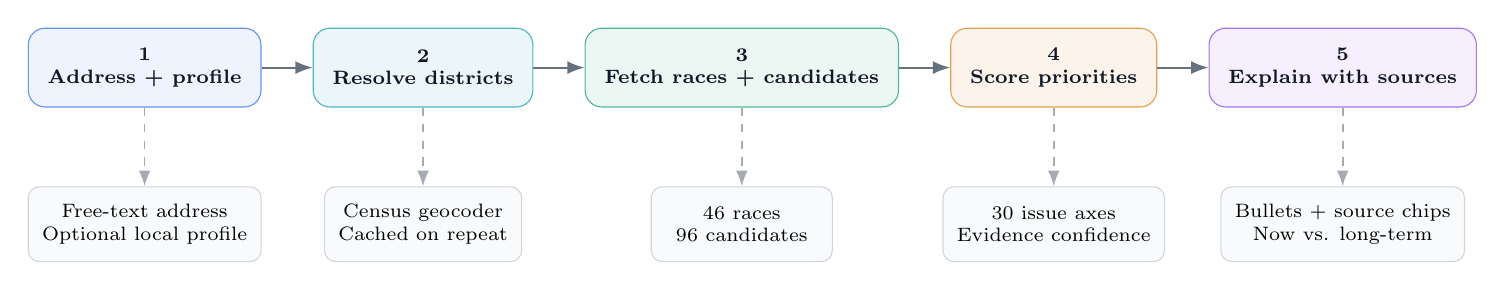
\begin{tikzpicture}[node distance=0.65cm]
    \node[service=blue,minimum width=2.3cm,minimum height=1.0cm] (step1) {1\\Address + profile};
    \node[service=cyan,right=of step1,minimum width=2.3cm,minimum height=1.0cm] (step2) {2\\Resolve districts};
    \node[service=green,right=of step2,minimum width=2.3cm,minimum height=1.0cm] (step3) {3\\Fetch races + candidates};
    \node[service=amber,right=of step3,minimum width=2.3cm,minimum height=1.0cm] (step4) {4\\Score priorities};
    \node[service=violet,right=of step4,minimum width=2.3cm,minimum height=1.0cm] (step5) {5\\Explain with sources};
    \draw[flow] (step1) -- (step2);
    \draw[flow] (step2) -- (step3);
    \draw[flow] (step3) -- (step4);
    \draw[flow] (step4) -- (step5);

    \node[lane,below=1.0cm of step1,minimum width=2.3cm] (p1) {Free-text address\\Optional local profile};
    \node[lane,below=1.0cm of step2,minimum width=2.3cm] (p2) {Census geocoder\\Cached on repeat};
    \node[lane,below=1.0cm of step3,minimum width=2.3cm] (p3) {46 races\\96 candidates};
    \node[lane,below=1.0cm of step4,minimum width=2.3cm] (p4) {30 issue axes\\Evidence confidence};
    \node[lane,below=1.0cm of step5,minimum width=2.3cm] (p5) {Bullets + source chips\\Now vs. long-term};
    \draw[softflow] (step1) -- (p1);
    \draw[softflow] (step2) -- (p2);
    \draw[softflow] (step3) -- (p3);
    \draw[softflow] (step4) -- (p4);
    \draw[softflow] (step5) -- (p5);
  \end{tikzpicture}%
  }

  \vspace{0.45cm}
  \begin{center}
    \chip{green}{Neutral comparison, not endorsement}
    \chip{red}{Missing data is a displayed measurement gap}
    \chip{blue}{Runtime hot path stays mostly cache reads}
  \end{center}
\end{frame}

\begin{frame}{Two-Service Monorepo}
  \centering
  \resizebox{\textwidth}{!}{%
  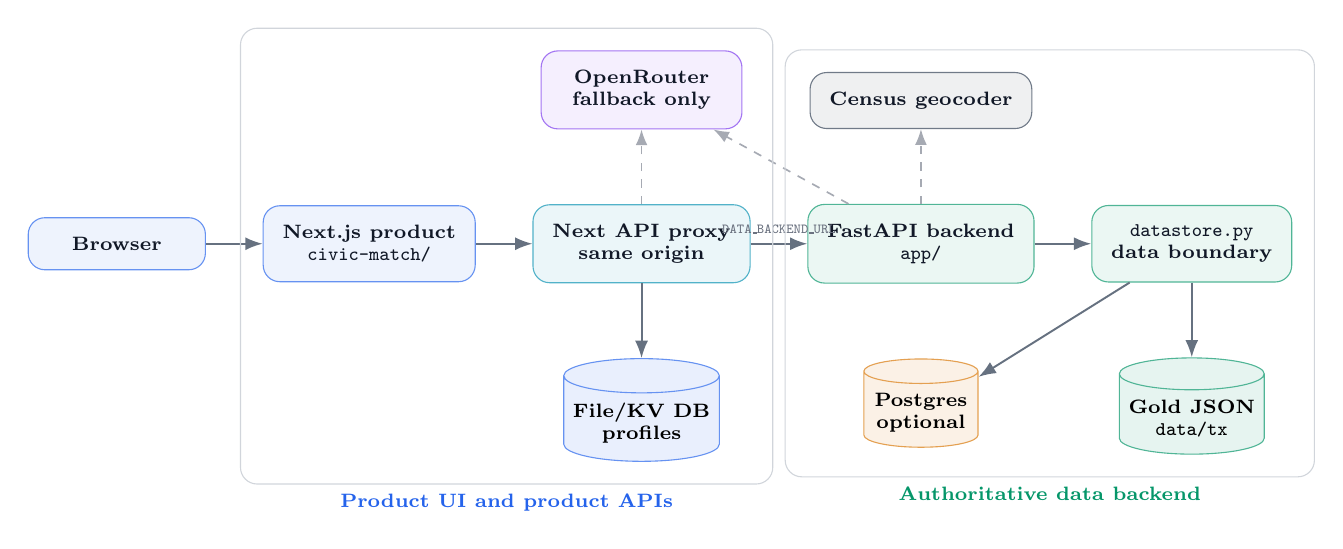
\begin{tikzpicture}[node distance=0.72cm]
    \node[service=blue,minimum width=2.25cm] (browser) {Browser};
    \node[service=blue,right=of browser,minimum width=2.55cm] (next) {Next.js product\\\texttt{civic-match/}};
    \node[service=cyan,right=of next,minimum width=2.55cm] (api) {Next API proxy\\same origin};
    \node[service=green,right=of api,minimum width=2.55cm] (fastapi) {FastAPI backend\\\texttt{app/}};
    \node[service=green,right=of fastapi,minimum width=2.30cm] (datastore) {\texttt{datastore.py}\\data boundary};

    \node[store=green,below=0.95cm of datastore] (json) {Gold JSON\\\texttt{data/tx}};
    \node[store=blue,below=0.95cm of api] (kv) {File/KV DB\\profiles};
    \node[store=amber,below=0.95cm of fastapi] (pg) {Postgres\\optional};
    \node[service=slate,above=0.95cm of fastapi,minimum width=2.55cm] (census) {Census geocoder};
    \node[service=violet,above=0.95cm of api,minimum width=2.55cm] (openrouter) {OpenRouter\\fallback only};

    \draw[flow] (browser) -- (next);
    \draw[flow] (next) -- (api);
    \draw[flow] (api) -- node[above,font=\tiny\color{muted}]{\texttt{DATA\_BACKEND\_URL}} (fastapi);
    \draw[flow] (fastapi) -- (datastore);
    \draw[flow] (datastore) -- (json);
    \draw[flow] (datastore) -- (pg);
    \draw[flow] (api) -- (kv);
    \draw[softflow] (fastapi) -- (census);
    \draw[softflow] (api) -- (openrouter);
    \draw[softflow] (fastapi) -- (openrouter);

    \node[draw=line,rounded corners=6pt,fit=(next)(api)(kv)(openrouter),inner sep=8pt,label={[font=\scriptsize\bfseries\color{blue}]below:Product UI and product APIs}] {};
    \node[draw=line,rounded corners=6pt,fit=(fastapi)(datastore)(json)(pg)(census),inner sep=8pt,label={[font=\scriptsize\bfseries\color{green}]below:Authoritative data backend}] {};
  \end{tikzpicture}%
  }
\end{frame}

\begin{frame}{Live Codebase Snapshot}
  \begin{columns}[T,onlytextwidth]
    \begin{column}{0.50\textwidth}
      \resizebox{\linewidth}{!}{%
      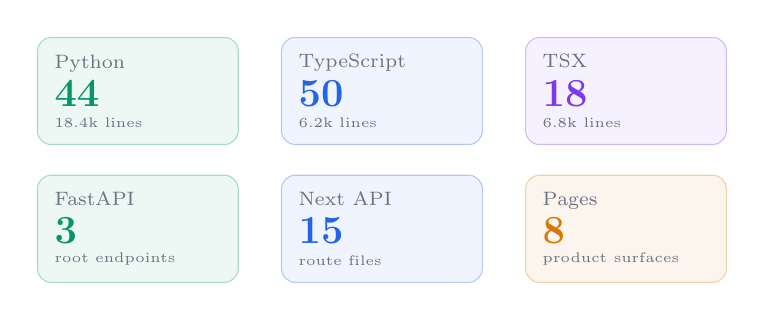
\begin{tikzpicture}
        \node at (0,0) {\statcard{green}{Python}{44}{18.4k lines}};
        \node at (3.1,0) {\statcard{blue}{TypeScript}{50}{6.2k lines}};
        \node at (6.2,0) {\statcard{violet}{TSX}{18}{6.8k lines}};
        \node at (0,-1.75) {\statcard{green}{FastAPI}{3}{root endpoints}};
        \node at (3.1,-1.75) {\statcard{blue}{Next API}{15}{route files}};
        \node at (6.2,-1.75) {\statcard{amber}{Pages}{8}{product surfaces}};
      \end{tikzpicture}%
      }
    \end{column}
    \begin{column}{0.48\textwidth}
      \scriptsize
      \begin{tabularx}{\linewidth}{>{\bfseries}p{1.45cm} X}
        \toprule
        Area & Main files inspected \\
        \midrule
        Backend & \texttt{main.py}, \texttt{datastore.py}, \texttt{insights.py}, \texttt{middleware.py} \\
        Pipeline & dataset build, Postgres load, horizons, validators \\
        Frontend & App Router pages, scoring, store, agents, data backend bridge \\
    Contracts & schema, frontend schemas, demo playbook \\
        \bottomrule
      \end{tabularx}

      \vspace{0.35cm}
      \chip{blue}{Repository root = data backend}
      \chip{green}{\texttt{civic-match/} = product frontend}
    \end{column}
  \end{columns}
\end{frame}

\begin{frame}{Gold Data Snapshot}
  \begin{columns}[T,onlytextwidth]
    \begin{column}{0.46\textwidth}
      \resizebox{\linewidth}{!}{%
      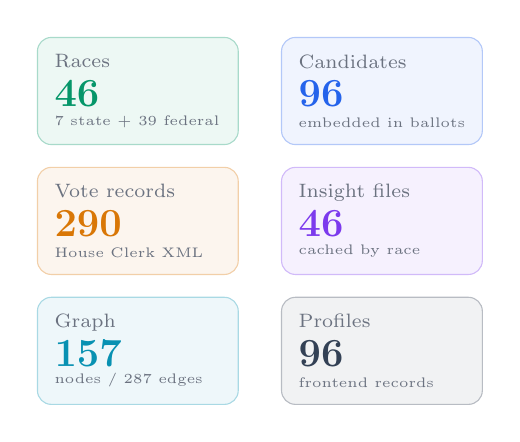
\begin{tikzpicture}
        \node at (0,0) {\statcard{green}{Races}{46}{7 state + 39 federal}};
        \node at (3.1,0) {\statcard{blue}{Candidates}{96}{embedded in ballots}};
        \node at (0,-1.65) {\statcard{amber}{Vote records}{290}{House Clerk XML}};
        \node at (3.1,-1.65) {\statcard{violet}{Insight files}{46}{cached by race}};
        \node at (0,-3.30) {\statcard{cyan}{Graph}{157}{nodes / 287 edges}};
        \node at (3.1,-3.30) {\statcard{slate}{Profiles}{96}{frontend records}};
      \end{tikzpicture}%
      }
    \end{column}
    \begin{column}{0.52\textwidth}
      \resizebox{\linewidth}{!}{%
      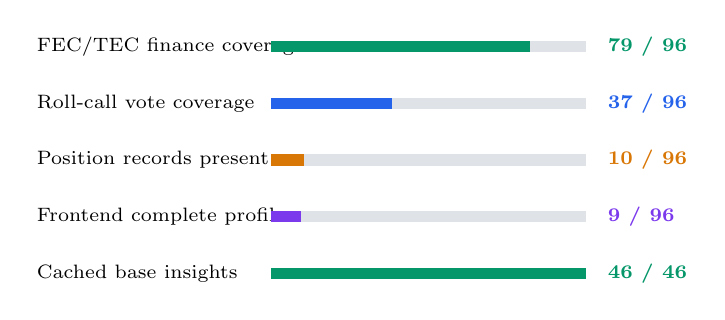
\begin{tikzpicture}[x=1cm,y=0.72cm]
        \barrow{0}{FEC/TEC finance coverage}{82.3}{79 / 96}{green}
        \barrow{-1}{Roll-call vote coverage}{38.5}{37 / 96}{blue}
        \barrow{-2}{Position records present}{10.4}{10 / 96}{amber}
        \barrow{-3}{Frontend complete profiles}{9.4}{9 / 96}{violet}
        \barrow{-4}{Cached base insights}{100}{46 / 46}{green}
      \end{tikzpicture}%
      }

      \vspace{0.25cm}
      \scriptsize\color{muted}
      Expanded reference layer in \texttt{data/politicians/}: 537 Congress members, 7,453 state legislators, and 76 Texas municipal officials.
    \end{column}
  \end{columns}
\end{frame}

\begin{frame}{Data Pipeline: Bronze to Runtime}
  \centering
  \resizebox{\textwidth}{!}{%
  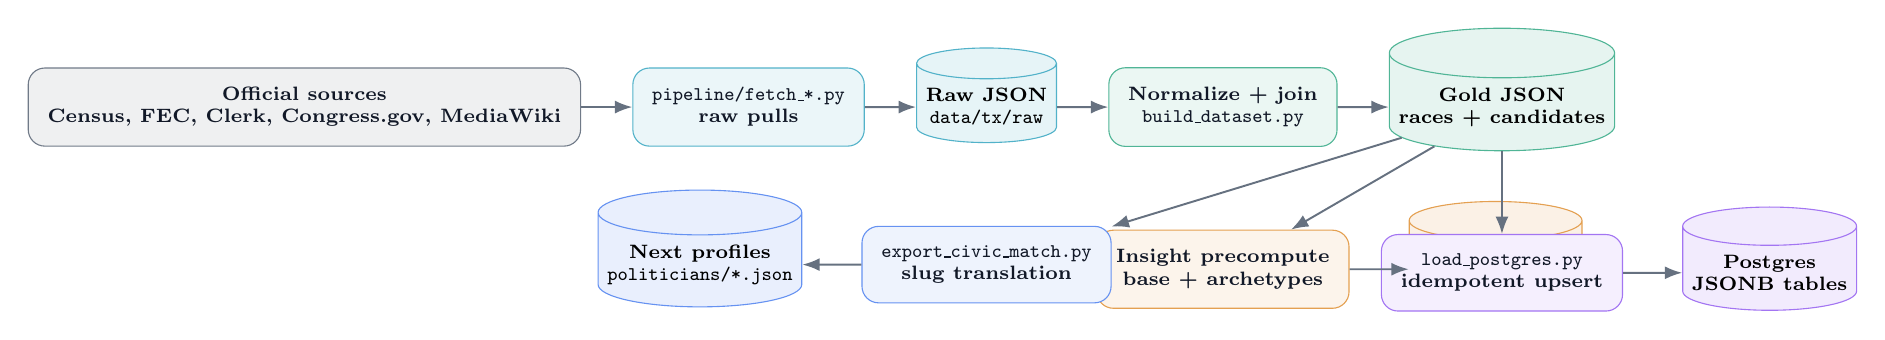
\begin{tikzpicture}[node distance=0.65cm]
    \node[service=slate,minimum width=2.55cm] (sources) {Official sources\\Census, FEC, Clerk, Congress.gov, MediaWiki};
    \node[service=cyan,right=of sources,minimum width=2.50cm] (fetch) {\texttt{pipeline/fetch\_*.py}\\raw pulls};
    \node[store=cyan,right=of fetch] (bronze) {Raw JSON\\\texttt{data/tx/raw}};
    \node[service=green,right=of bronze,minimum width=2.55cm] (build) {Normalize + join\\\texttt{build\_dataset.py}};
    \node[store=green,right=of build] (gold) {Gold JSON\\races + candidates};

    \node[service=amber,below=1.05cm of build,minimum width=2.75cm] (insight) {Insight precompute\\base + archetypes};
    \node[store=amber,right=0.75cm of insight] (insightfiles) {\texttt{data/tx/}\\\texttt{insights/*.json}};
    \node[service=violet,below=1.05cm of gold,minimum width=2.50cm] (pgload) {\texttt{load\_postgres.py}\\idempotent upsert};
    \node[store=violet,right=0.75cm of pgload] (postgres) {Postgres\\JSONB tables};
    \node[service=blue,below=1.05cm of bronze,minimum width=2.50cm] (export) {\texttt{export\_civic\_match.py}\\slug translation};
    \node[store=blue,left=0.75cm of export] (profiles) {Next profiles\\\texttt{politicians/*.json}};

    \draw[flow] (sources) -- (fetch);
    \draw[flow] (fetch) -- (bronze);
    \draw[flow] (bronze) -- (build);
    \draw[flow] (build) -- (gold);
    \draw[flow] (gold) -- (insight);
    \draw[flow] (insight) -- (insightfiles);
    \draw[flow] (gold) -- (pgload);
    \draw[flow] (pgload) -- (postgres);
    \draw[flow] (gold) -- (export);
    \draw[flow] (export) -- (profiles);
  \end{tikzpicture}%
  }

  \vspace{0.2cm}
  \begin{center}
    \chip{green}{Gold files are source of truth}
    \chip{amber}{Runtime selects cached insight blocks}
    \chip{violet}{Postgres is production path, JSON fallback stays functional}
  \end{center}
\end{frame}

\begin{frame}{Ballot Hot Path}
  \centering
  \resizebox{\textwidth}{!}{%
  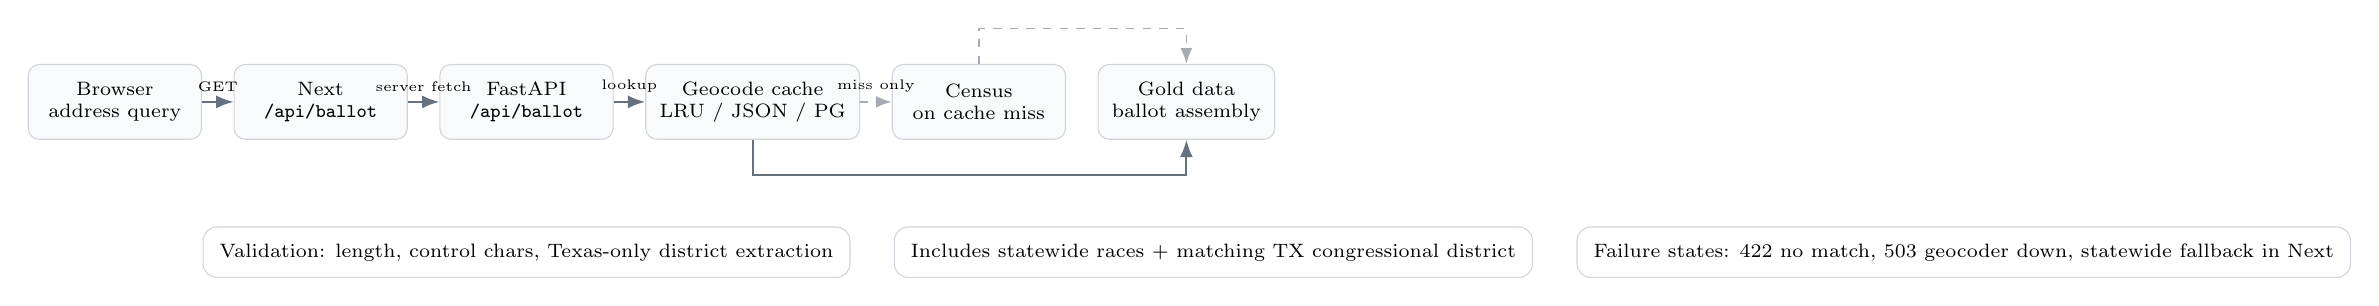
\begin{tikzpicture}[node distance=0.40cm]
    \node[lane,minimum width=2.2cm] (browser) {Browser\\address query};
    \node[lane,right=of browser,minimum width=2.2cm] (next) {Next\\\texttt{/api/ballot}};
    \node[lane,right=of next,minimum width=2.2cm] (fastapi) {FastAPI\\\texttt{/api/ballot}};
    \node[lane,right=of fastapi,minimum width=2.2cm] (cache) {Geocode cache\\LRU / JSON / PG};
    \node[lane,right=of cache,minimum width=2.2cm] (census) {Census\\on cache miss};
    \node[lane,right=of census,minimum width=2.2cm] (gold) {Gold data\\ballot assembly};

    \draw[flow] (browser) -- node[above,font=\tiny]{GET} (next);
    \draw[flow] (next) -- node[above,font=\tiny]{server fetch} (fastapi);
    \draw[flow] (fastapi) -- node[above,font=\tiny]{lookup} (cache);
    \draw[softflow] (cache) -- node[above,font=\tiny]{miss only} (census);
    \draw[flow] (cache) |- ($(gold.south)+(0,-0.45)$) -| (gold);
    \draw[softflow] (census) |- ($(gold.north)+(0,0.45)$) -| (gold);

    \node[box,below=1.10cm of fastapi,minimum width=3.6cm] (validate) {Validation: length, control chars, Texas-only district extraction};
    \node[box,right=0.55cm of validate,minimum width=3.6cm] (races) {Includes statewide races + matching TX congressional district};
    \node[box,right=0.55cm of races,minimum width=3.6cm] (warn) {Failure states: 422 no match, 503 geocoder down, statewide fallback in Next};
  \end{tikzpicture}%
  }
\end{frame}

\begin{frame}{Insight Safety Boundary}
  \centering
  \resizebox{\textwidth}{!}{%
  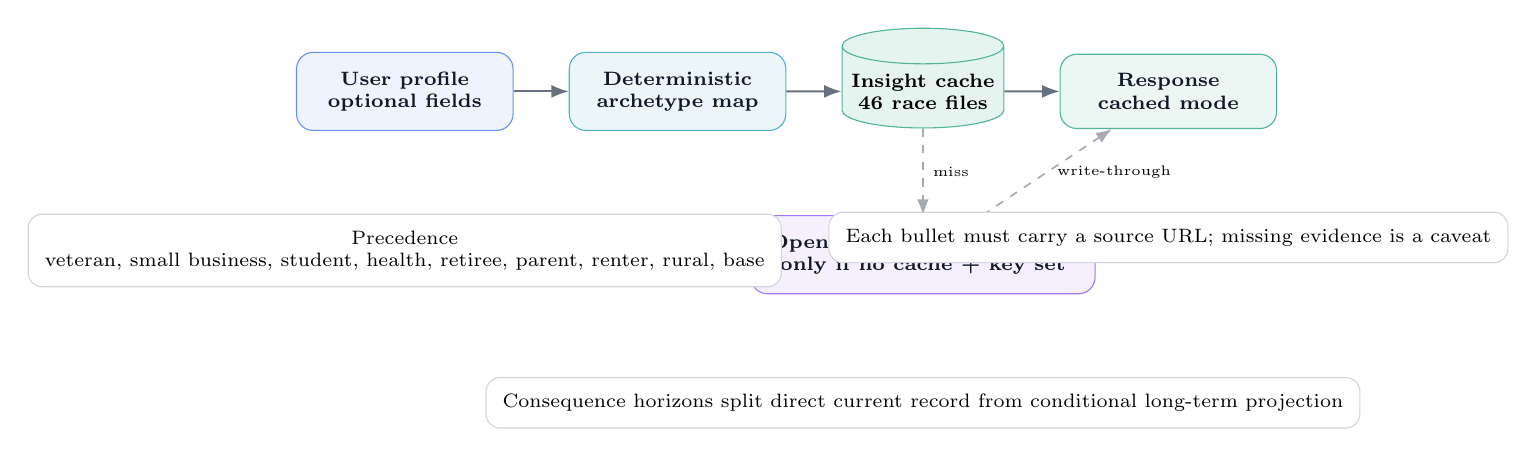
\begin{tikzpicture}[node distance=0.70cm]
    \node[service=blue,minimum width=2.75cm] (profile) {User profile\\optional fields};
    \node[service=cyan,right=of profile,minimum width=2.75cm] (map) {Deterministic\\archetype map};
    \node[store=green,right=of map] (cache) {Insight cache\\46 race files};
    \node[service=green,right=of cache,minimum width=2.75cm] (response) {Response\\cached mode};
    \draw[flow] (profile) -- (map);
    \draw[flow] (map) -- (cache);
    \draw[flow] (cache) -- (response);

    \node[service=violet,below=1.10cm of cache,minimum width=3.0cm] (llm) {OpenRouter live generation\\only if no cache + key set};
    \draw[softflow] (cache) -- node[right,font=\tiny]{miss} (llm);
    \draw[softflow] (llm) -- node[right,font=\tiny]{write-through} (response);

    \node[box,below=1.05cm of profile,minimum width=3.1cm] {Precedence\\veteran, small business, student, health, retiree, parent, renter, rural, base};
    \node[box,below=1.05cm of response,minimum width=3.1cm] {Each bullet must carry a source URL; missing evidence is a caveat};
    \node[box,below=1.05cm of llm,minimum width=3.1cm] {Consequence horizons split direct current record from conditional long-term projection};
  \end{tikzpicture}%
  }

  \vspace{0.35cm}
  \begin{center}
    \chip{green}{Base insights: 46 / 46 races}
    \chip{amber}{Eight voter archetypes cached for 10 marquee races}
    \chip{red}{No key means unavailable, not fabricated}
  \end{center}
\end{frame}

\begin{frame}{Evidence Machine}
  \centering
  \resizebox{0.96\textwidth}{!}{%
  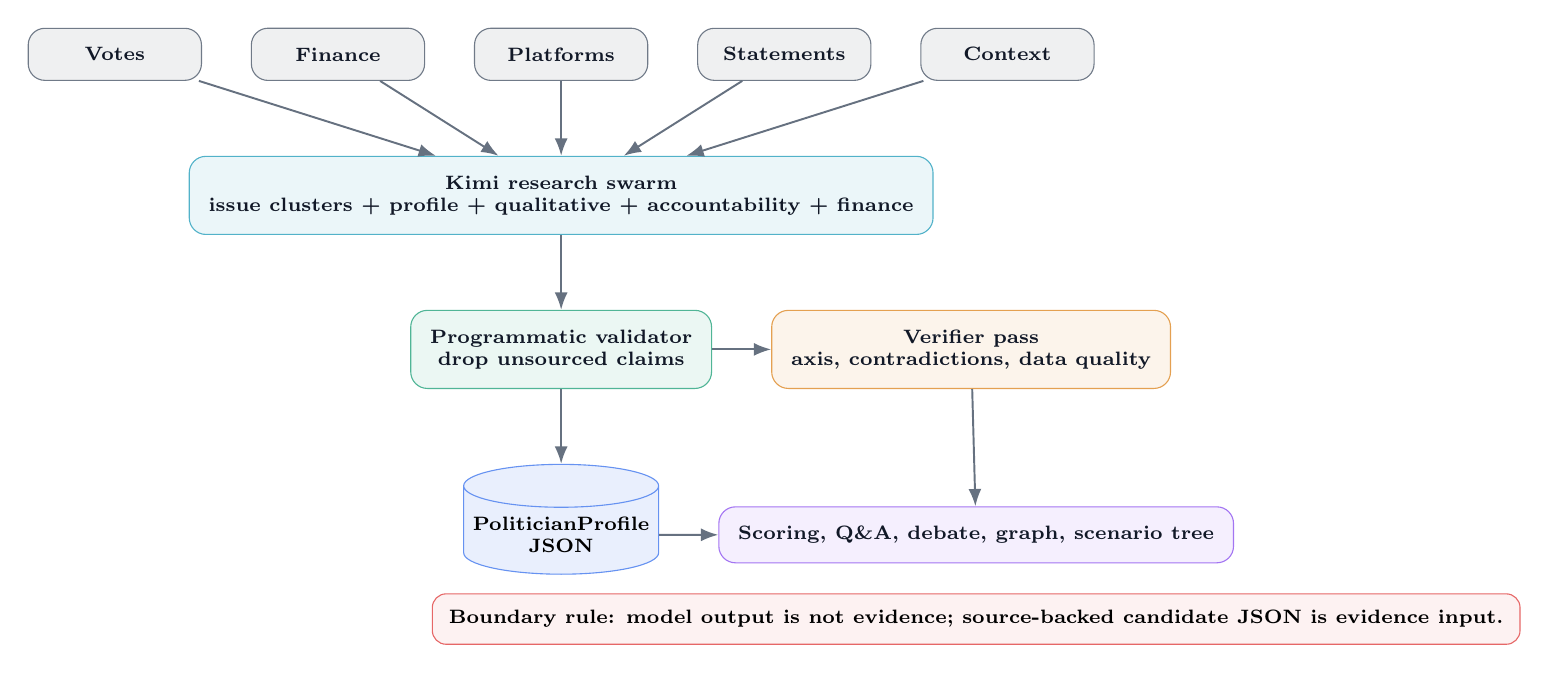
\begin{tikzpicture}[node distance=0.62cm]
    \node[service=slate,minimum width=2.20cm] (votes) {Votes};
    \node[service=slate,right=of votes,minimum width=2.20cm] (finance) {Finance};
    \node[service=slate,right=of finance,minimum width=2.20cm] (platform) {Platforms};
    \node[service=slate,right=of platform,minimum width=2.20cm] (statements) {Statements};
    \node[service=slate,right=of statements,minimum width=2.20cm] (context) {Context};

    \node[service=cyan,below=0.95cm of platform,minimum width=4.15cm] (agents) {Kimi research swarm\\issue clusters + profile + qualitative + accountability + finance};
    \node[service=green,below=0.95cm of agents,minimum width=3.1cm] (validator) {Programmatic validator\\drop unsourced claims};
    \node[service=amber,right=0.75cm of validator,minimum width=3.1cm] (verifier) {Verifier pass\\axis, contradictions, data quality};
    \node[store=blue,below=0.95cm of validator] (profiles) {PoliticianProfile\\JSON};
    \node[service=violet,right=0.75cm of profiles,minimum width=3.1cm] (surfaces) {Scoring, Q\&A, debate, graph, scenario tree};

    \draw[flow] (votes) -- (agents);
    \draw[flow] (finance) -- (agents);
    \draw[flow] (platform) -- (agents);
    \draw[flow] (statements) -- (agents);
    \draw[flow] (context) -- (agents);
    \draw[flow] (agents) -- (validator);
    \draw[flow] (validator) -- (verifier);
    \draw[flow] (validator) -- (profiles);
    \draw[flow] (verifier) -- (surfaces);
    \draw[flow] (profiles) -- (surfaces);

    \node[draw=red!70,fill=red!6,rounded corners=5pt,inner sep=6pt,align=center,font=\scriptsize\bfseries,below=0.38cm of surfaces,minimum width=5.0cm] {Boundary rule: model output is not evidence; source-backed candidate JSON is evidence input.};
  \end{tikzpicture}%
  }
\end{frame}

\begin{frame}{Scoring: Auditable Math}
  \begin{columns}[T,onlytextwidth]
    \begin{column}{0.48\textwidth}
      \small
      \begin{block}{Issue alignment}
        \[
          \sum w_i \times a_i \times c_i \times r_i \times q_i
        \]
        \vspace{-0.2cm}
        \begin{tabularx}{\linewidth}{>{\bfseries}l X}
          \(w_i\) & user's normalized priority weight \\
          \(a_i\) & scalar closeness: \(1-|user-candidate|\) \\
          \(c_i\) & evidence confidence \\
          \(r_i\) & recency adjustment \\
          \(q_i\) & source quality multiplier \\
        \end{tabularx}
      \end{block}
      \chip{red}{Unknown evidence lowers confidence, not alignment}
    \end{column}
    \begin{column}{0.50\textwidth}
      \resizebox{\linewidth}{!}{%
      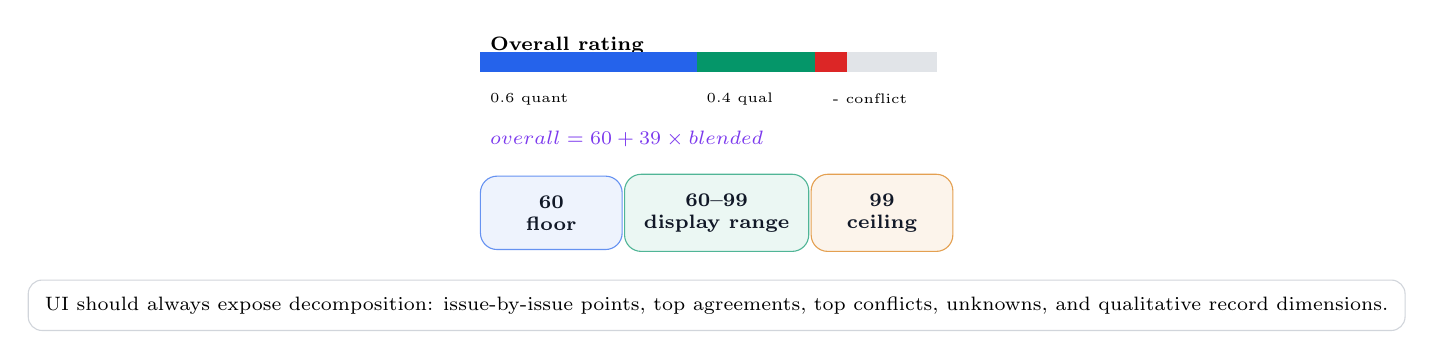
\begin{tikzpicture}[x=1cm,y=0.85cm]
        \node[anchor=west,font=\scriptsize\bfseries] at (0,0.25) {Overall rating};
        \fill[line!65] (0,-0.15) rectangle (5.8,0.15);
        \fill[blue] (0,-0.15) rectangle (2.75,0.15);
        \fill[green] (2.75,-0.15) rectangle (4.65,0.15);
        \fill[red] (4.65,-0.15) rectangle (4.25,0.15);
        \node[anchor=west,font=\tiny] at (0,-0.55) {0.6 quant};
        \node[anchor=west,font=\tiny] at (2.75,-0.55) {0.4 qual};
        \node[anchor=west,font=\tiny] at (4.35,-0.55) {- conflict};
        \node[anchor=west,font=\scriptsize\bfseries\color{violet}] at (0,-1.15) {\(\text{overall}=60+39\times blended\)};

        \node[service=blue,minimum width=1.8cm] at (0.9,-2.25) {60\\floor};
        \node[service=green,minimum width=1.8cm] at (3.0,-2.25) {60--99\\display range};
        \node[service=amber,minimum width=1.8cm] at (5.1,-2.25) {99\\ceiling};

        \node[box,minimum width=5.8cm,below=0.35cm of current bounding box.south] {UI should always expose decomposition: issue-by-issue points, top agreements, top conflicts, unknowns, and qualitative record dimensions.};
      \end{tikzpicture}%
      }
    \end{column}
  \end{columns}
\end{frame}

\begin{frame}{Product Surface Map}
  \centering
  \resizebox{\textwidth}{!}{%
  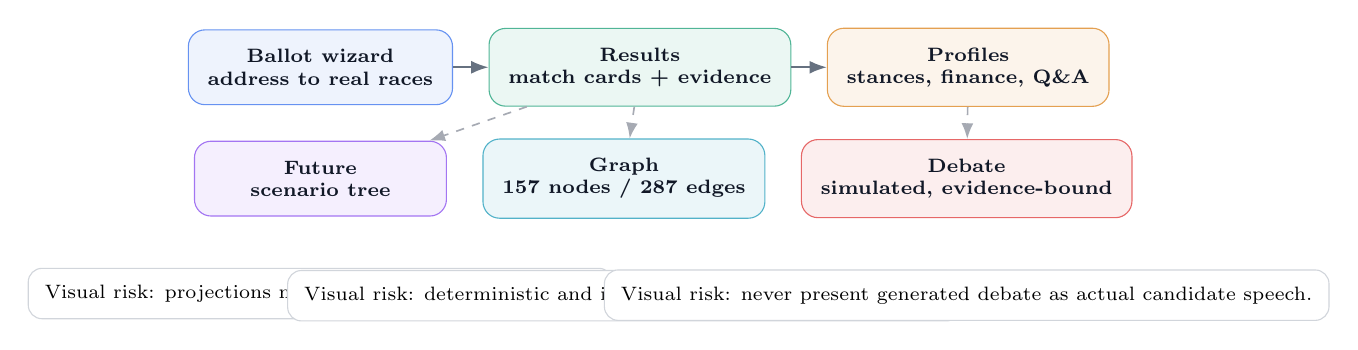
\begin{tikzpicture}[node distance=0.45cm]
    \node[service=blue,minimum width=3.20cm,minimum height=0.95cm] (ballot) {Ballot wizard\\address to real races};
    \node[service=green,right=of ballot,minimum width=3.20cm,minimum height=0.95cm] (results) {Results\\match cards + evidence};
    \node[service=amber,right=of results,minimum width=3.20cm,minimum height=0.95cm] (profile) {Profiles\\stances, finance, Q\&A};
    \node[service=violet,below=of ballot,minimum width=3.20cm,minimum height=0.95cm] (future) {Future\\scenario tree};
    \node[service=cyan,right=of future,minimum width=3.20cm,minimum height=0.95cm] (graph) {Graph\\157 nodes / 287 edges};
    \node[service=red,right=of graph,minimum width=3.20cm,minimum height=0.95cm] (debate) {Debate\\simulated, evidence-bound};

    \node[box,below=0.65cm of future,minimum width=3.20cm] {Visual risk: projections must stay labeled as projections.};
    \node[box,below=0.65cm of graph,minimum width=3.20cm] {Visual risk: deterministic and inferred edges need distinct styling.};
    \node[box,below=0.65cm of debate,minimum width=3.20cm] {Visual risk: never present generated debate as actual candidate speech.};

    \draw[flow] (ballot) -- (results);
    \draw[flow] (results) -- (profile);
    \draw[softflow] (results) -- (future);
    \draw[softflow] (results) -- (graph);
    \draw[softflow] (profile) -- (debate);
  \end{tikzpicture}%
  }
\end{frame}

\begin{frame}{API and Data Boundaries}
  \scriptsize
  \begin{tabularx}{\linewidth}{>{\bfseries}p{2.25cm} p{2.75cm} X}
    \toprule
    Boundary & Endpoint or module & Presentation-safe claim \\
    \midrule
    Backend health & \texttt{GET /healthz} & Reports data-loaded status plus race, candidate, and insight counts. \\
    Ballot lookup & \texttt{GET /api/ballot} & Texas address resolves to districts, then statewide plus district-specific races. \\
    Insights & \texttt{POST /api/insights} & Picks cached archetype block before any live model fallback. \\
    Next proxy & \texttt{app/api/ballot} & Browser talks same-origin Next; backend URL stays server-side. \\
    Voter insights & \texttt{/api/voter-insights} & Translates frontend profile shape to backend archetype contract. \\
    Research & research + check & SSE research flow for insufficient candidate data. \\
    Storage & datastore + store & Backend uses Postgres-or-JSON; frontend uses KV Postgres-or-file DB. \\
    \bottomrule
  \end{tabularx}

  \vspace{0.35cm}
  \begin{center}
    \chip{green}{HTTP handlers do not own storage details}
    \chip{blue}{Data access has explicit fallback paths}
    \chip{red}{Addresses and profiles are request-local, not stored as user accounts}
  \end{center}
\end{frame}

\begin{frame}{Demo Path in Three Minutes}
  \centering
  \resizebox{\textwidth}{!}{%
  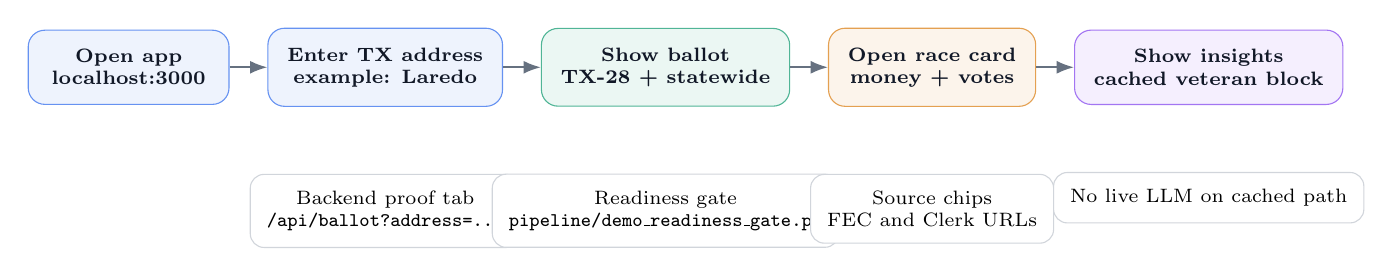
\begin{tikzpicture}[node distance=0.48cm]
    \node[service=blue,minimum width=2.55cm] (home) {Open app\\localhost:3000};
    \node[service=blue,right=of home,minimum width=2.55cm] (address) {Enter TX address\\example: Laredo};
    \node[service=green,right=of address,minimum width=2.55cm] (ballot) {Show ballot\\TX-28 + statewide};
    \node[service=amber,right=of ballot,minimum width=2.55cm] (card) {Open race card\\money + votes};
    \node[service=violet,right=of card,minimum width=2.55cm] (insights) {Show insights\\cached veteran block};

    \draw[flow] (home) -- (address);
    \draw[flow] (address) -- (ballot);
    \draw[flow] (ballot) -- (card);
    \draw[flow] (card) -- (insights);

    \node[box,below=0.85cm of address,minimum width=3.05cm] {Backend proof tab\\\texttt{/api/ballot?address=...}};
    \node[box,below=0.85cm of ballot,minimum width=3.05cm] {Readiness gate\\\texttt{pipeline/demo\_readiness\_gate.py}};
    \node[box,below=0.85cm of card,minimum width=3.05cm] {Source chips\\FEC and Clerk URLs};
    \node[box,below=0.85cm of insights,minimum width=3.05cm] {No live LLM on cached path};
  \end{tikzpicture}%
  }

  \vspace{0.35cm}
  \begin{center}
    \chip{green}{46 races}
    \chip{green}{96 candidates}
    \chip{green}{290 vote records}
    \chip{amber}{Railway backend + JSON fallback}
  \end{center}
\end{frame}

\begin{frame}{What We Can Defend to Judges}
  \begin{columns}[T,onlytextwidth]
    \begin{column}{0.48\textwidth}
      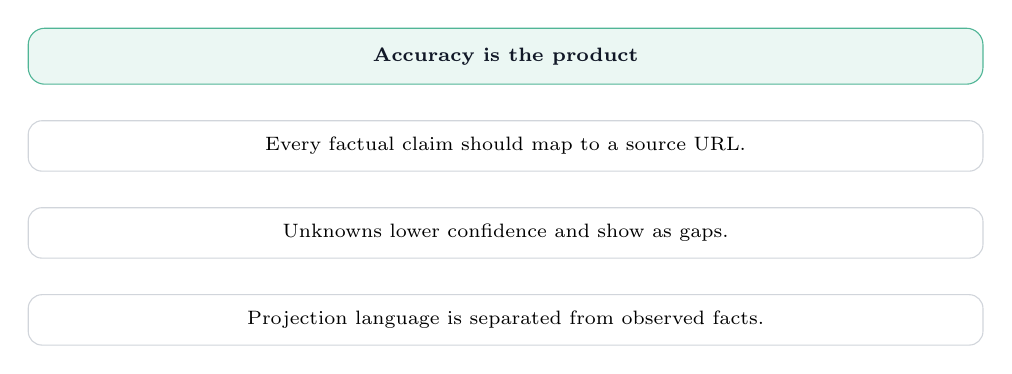
\begin{tikzpicture}[node distance=0.45cm]
        \node[service=green,minimum width=\linewidth] (a) {Accuracy is the product};
        \node[box,below=of a,minimum width=\linewidth] (b) {Every factual claim should map to a source URL.};
        \node[box,below=of b,minimum width=\linewidth] (c) {Unknowns lower confidence and show as gaps.};
        \node[box,below=of c,minimum width=\linewidth] (d) {Projection language is separated from observed facts.};
      \end{tikzpicture}
    \end{column}
    \begin{column}{0.48\textwidth}
      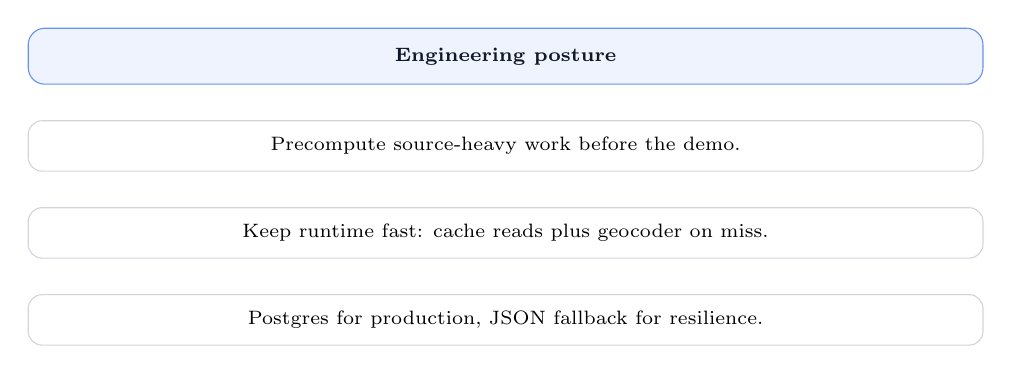
\begin{tikzpicture}[node distance=0.45cm]
        \node[service=blue,minimum width=\linewidth] (a) {Engineering posture};
        \node[box,below=of a,minimum width=\linewidth] (b) {Precompute source-heavy work before the demo.};
        \node[box,below=of b,minimum width=\linewidth] (c) {Keep runtime fast: cache reads plus geocoder on miss.};
        \node[box,below=of c,minimum width=\linewidth] (d) {Postgres for production, JSON fallback for resilience.};
      \end{tikzpicture}
    \end{column}
  \end{columns}

  \vspace{0.45cm}
  \begin{center}
    {\Large\bfseries One-line close}\\[0.12cm]
    {\color{muted}Civic Match turns a Texas address into a sourced ballot explanation, while making the evidence boundary visible at every step.}
  \end{center}
\end{frame}

\appendix

\begin{frame}{Appendix: Current Route Inventory}
  \scriptsize
  \begin{tabularx}{\linewidth}{>{\bfseries}p{2.35cm} p{1.7cm} X}
    \toprule
    Surface & Method & Purpose \\
    \midrule
    FastAPI \texttt{/healthz} & GET & Healthcheck and data counts. \\
    FastAPI \texttt{/api/ballot} & GET & Address validation, geocoding, district extraction, ballot assembly. \\
    FastAPI \texttt{/api/insights} & POST & Archetype mapping, cached insights, optional OpenRouter fallback. \\
    Next \texttt{/api/ballot} & GET & Same-origin proxy with statewide fallback. \\
    Next \texttt{/api/match} & POST & Pure scoring over cached profiles. \\
    Next \texttt{/api/research} & POST & SSE candidate research flow. \\
    Next \texttt{check-research} & GET & Insufficient-data detection for one-click research. \\
    Next Q\&A / explain / debate & POST & Evidence-bounded generated product surfaces. \\
    Next graph / scenario / stakes & GET & Visual civic context layers. \\
    \bottomrule
  \end{tabularx}
\end{frame}

\end{document}
